\section{Database Design}
MongoDB is used for \serviceName, using MongoDB Atlas as the database provider.

The database currently looks like this:
\begin{figure}[ht]
    \centering
    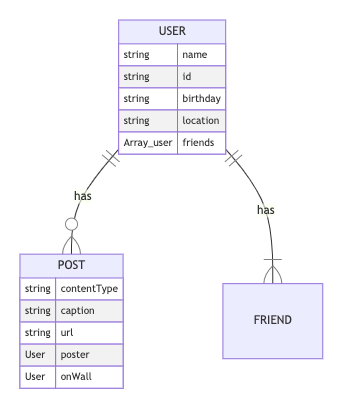
\includegraphics[scale=0.5]{twine-erd.png}
    \caption{\serviceName ERD}
    \label{}
\end{figure}

\section{User Journey}
The User Journey will look like this:

\begin{figure}[ht]
    \centering
    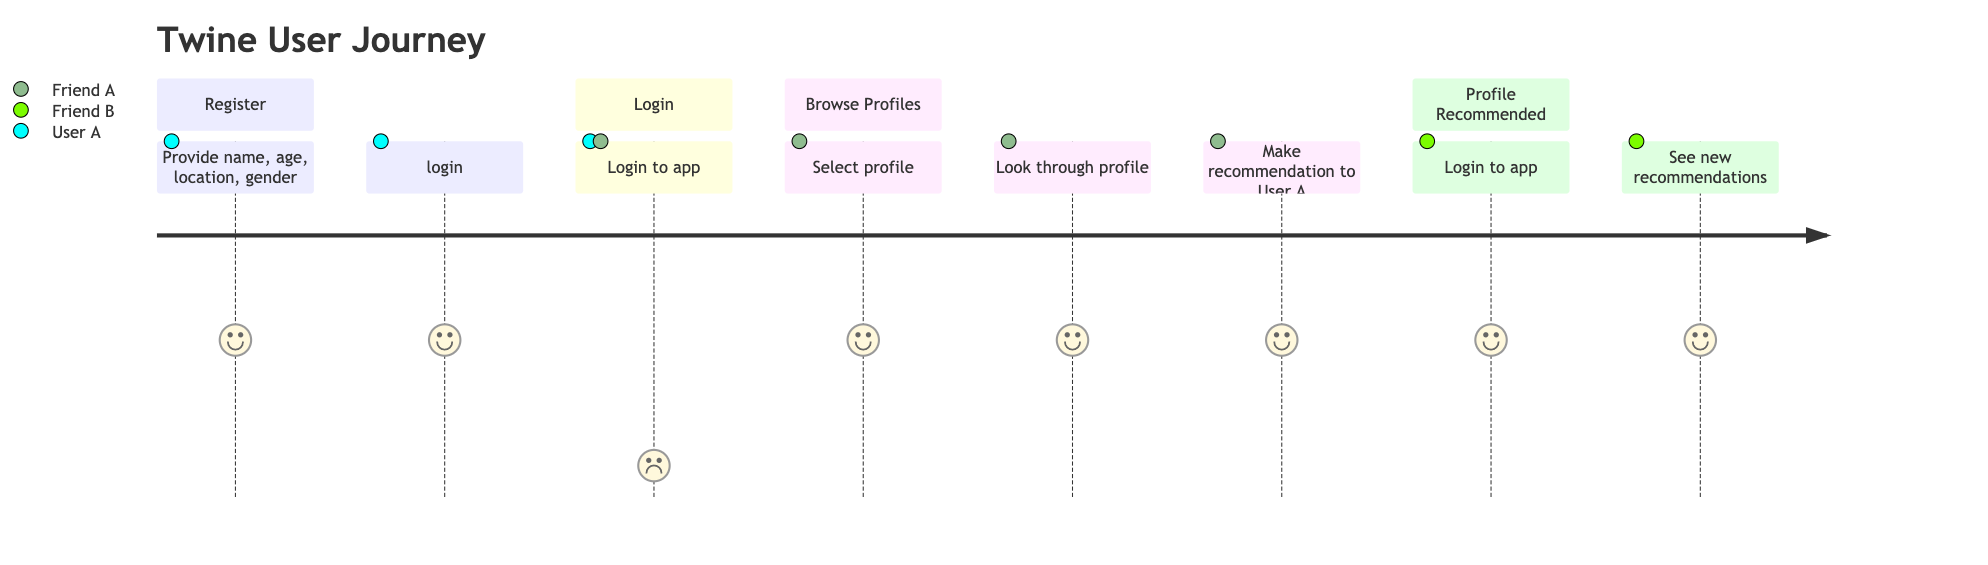
\includegraphics[scale=0.2]{twine-user-journey.png}
    \caption{\serviceName user model}
    \label{find use}
\end{figure}

\section{Data Interaction}
\serviceName will read and write to a MongoDB database via an API written in ExpressJS. The API will communicate
with a ReactJS frontend.